%\documentclass[12pt]{article}
\documentclass[12pt]{scrartcl}
\title{DA6400 Assignment 3}
\nonstopmode
%\usepackage[utf-8]{inputenc}
\usepackage{graphicx} % Required for including pictures
\usepackage[figurename=Figure]{caption}
\usepackage{float}    % For tables and other floats
\usepackage{verbatim} % For comments and other
\usepackage{amsmath}  % For math
\usepackage{amssymb}  % For more math
\usepackage[left=0.5in, right=0.5in, top=0.6in]{geometry}
\usepackage{paralist} % paragraph spacing
\usepackage{listings} % For source code
\usepackage{subcaption}
%\usepackage{physics}  % for simplified dv, and 
\usepackage{enumitem} % useful for itemization
\usepackage{siunitx}  % standardization of si units
\usepackage{hyperref}
\usepackage{tikz,bm} % Useful for drawing plots
%\usepackage{tikz-3dplot}
\usepackage{circuitikz}
\usepackage{placeins}
% Reduce spacing between paragraphs
\setlength{\parskip}{2pt} 

% Reduce spacing around floats (tables and figures)
% \setlength{\floatsep}{5pt plus 2pt minus 2pt}
% \setlength{\textfloatsep}{5pt plus 2pt minus 2pt}
% \setlength{\intextsep}{5pt plus 2pt minus 2pt}

% Condense lists (itemize/enumerate)
\setlist[enumerate]{topsep=2pt, itemsep=0pt, partopsep=0pt, parsep=0pt}
\setlist[itemize]{topsep=2pt, itemsep=0pt, partopsep=0pt, parsep=0pt}

%%% Colours used in field vectors and propagation direction
\definecolor{mycolor}{rgb}{1,0.2,0.3}
\definecolor{brightgreen}{rgb}{0.4, 1.0, 0.0}
\definecolor{britishracinggreen}{rgb}{0.0, 0.26, 0.15}
\definecolor{cadmiumgreen}{rgb}{0.0, 0.42, 0.24}
\definecolor{ceruleanblue}{rgb}{0.16, 0.32, 0.75}
\definecolor{darkelectricblue}{rgb}{0.33, 0.41, 0.47}
\definecolor{darkpowderblue}{rgb}{0.0, 0.2, 0.6}
\definecolor{darktangerine}{rgb}{1.0, 0.66, 0.07}
\definecolor{emerald}{rgb}{0.31, 0.78, 0.47}
\definecolor{palatinatepurple}{rgb}{0.41, 0.16, 0.38}
\definecolor{pastelviolet}{rgb}{0.8, 0.6, 0.79}
\begin{document}

\begin{center}
	\hrule
	\vspace{.4cm}
	{\textbf { \large DA6400 -- Assignment 3}}
\end{center}
{\textbf{Name:}\ Yash Purswani, Govind S Ashan, Tiramdas Abhinand \hspace{\fill} \textbf{Due Date:} May 8 2026, 11:59 PM   \\
{ \textbf{Student Number:}} \ ME22B214, ME23B168, ME23B208 \hspace{\fill} \textbf{Assignment:} 3 \\

\noindent \textbf{Division of Work:} Yash was responsible for tackling Questions 1, 2, and 3. Abhinand completed Question 4, while Govind handled Question 5.

\noindent The Google Drive link for the code can be found \href{link}{here}.

\url{link}}
\hrule

% ── Q1: Pendulum ─────────────────────────────────────────────────────────────
\paragraph*{Problem 1}
\begin{enumerate}
    \item \textbf{Reward Function Design:} The primary objective is to drive the pendulum to a specific target angle $\theta_{\text{target}}$ and stabilize it there indefinitely. To achieve this, we design a dense, smooth reward function that provides informative gradients across the entire state space:
    \begin{equation}
    R(s, a) = - \Delta\theta^2 - 0.1 \dot{\theta}^2 - 0.001 u^2
    \end{equation}
    The first term, $\Delta\theta^2$, where $\Delta\theta = \text{atan2}(\sin(\theta - \theta_{\text{target}}), \cos(\theta - \theta_{\text{target}}))$, serves as the position penalty. Using the $\text{atan2}$ formulation ensures that the agent always perceives the shortest angular path to the target, preventing unnecessary full rotations. Squaring the difference creates a parabolic cost landscape that is steepest far from the target and flat at the goal, providing a strong directive for the agent to move towards $\theta_{\text{target}}$.
    
    The second term, $- 0.1 \dot{\theta}^2$, is a crucial damping component. In a continuous control environment like the Pendulum, an agent rewarded solely on position would likely reach the target with high kinetic energy, leading to persistent oscillations or overshoot. By penalizing angular velocity, we encourage the agent to arrive at the target with zero momentum, facilitating a "soft landing" and steady-state stability.
    
    The final term, $- 0.001 u^2$, regularizes the control effort. It penalizes excessive torque (action $u$), which prevents the policy from exhibiting aggressive "bang-bang" control. This promotes energy efficiency and ensures a smoother, more realistic policy that avoids high-frequency chatter in the torque output, which is essential for the longevity of physical actuators.

    \item \textbf{SAC Implementation with Automated Tuning:} Soft Actor-Critic (SAC) is an off-policy actor-critic algorithm based on the maximum entropy reinforcement learning framework. Our implementation incorporates several key architectural features to ensure stable and efficient learning:
    \begin{itemize}
        \item \textbf{Squashed Gaussian Policy:} The actor outputs the mean and standard deviation of a Gaussian distribution. We apply the reparameterization trick ($a = f_\phi(\epsilon; s)$) to allow backpropagation through stochastic nodes. The resulting action is passed through a Tanh activation to squash it into the $[-1, 1]$ range, which is then scaled to the environment's torque limits.
        \item \textbf{Clipped Double-Q Learning:} To combat the well-known overestimation bias in Q-learning, we maintain two independent critic networks and use the minimum of their predictions for the policy and value updates. This conservative estimate prevents the agent from being trapped in sub-optimal "optimistic" local minima.
        \item \textbf{Automated Temperature Tuning:} Instead of a fixed entropy weight $\alpha$, we treat $\alpha$ as a learnable parameter. The agent optimizes $\alpha$ to maintain a target entropy $\bar{H} = -|\mathcal{A}| = -1$. This automation is critical because the relative scale of the reward and entropy bonus can shift dramatically during training; a learnable $\alpha$ ensures that exploration is prioritized early on while allowing the policy to become deterministic (exploitative) as it converges on the optimal behavior.
    \end{itemize}

    \item \textbf{Comparison of Results for Different $\theta_{\text{target}}$:} The experimental results demonstrate that the difficulty of the task is intrinsically linked to the physics of gravitational torque. 
    \begin{itemize}
        \item \textbf{Stable Equilibrium Targets ($\theta \approx \pm 180^\circ$):} Targets like $\theta = -150^\circ$ show the fastest convergence and highest returns (Best $\approx -80$). These positions are physically close to the natural hanging position where gravity assists in stabilization. The agent needs minimal torque to counteract gravity, allowing it to stay stationary with high precision.
        \item \textbf{Unstable Horizontal Targets ($\theta = \pm 90^\circ$):} These are the most challenging configurations. At $90^\circ$, the gravitational torque ($mgl \sin\theta$) is at its maximum. To maintain this position, the agent must apply a perfectly matched, constant torque. Any stochasticity in the policy (due to entropy) or lag in control leads to a deviation that gravity quickly amplifies, resulting in a large drop and severe penalty. This is reflected in the significantly lower returns (Last $\approx -1500$) and higher variance observed in the curves.
        \item \textbf{Upright Target ($\theta = 0^\circ$):} While gravity is zero at the vertical, the position is an unstable equilibrium. The agent must learn a delicate balance to stay upright, making it harder than the hanging positions but easier than the horizontal ones.
    \end{itemize}
    \begin{figure}[H]
        \centering
        
\includegraphics[width=0.9\textwidth]{images/sac_pendulum_plot.png}
        \caption{SAC performance for various target angles $\theta_{\text{target}}$ in Pendulum-v1. Note the significant performance gap between stable hanging positions and unstable horizontal targets.}
        \label{fig:sac_pendulum}
    \end{figure}

    \item \textbf{Optimal Behavior Analysis:} The optimal policy must master two distinct physical and behavioral regimes:
    \begin{enumerate}
        \item \textbf{Reachability (The Transient Phase):} This involves the dynamic swing-up (or swing-down) maneuver. The agent must understand the system's inertia and gravitational effects to reach $\theta_{\text{target}}$ efficiently. For targets far from the initial state, the agent may need to build momentum by swinging in the opposite direction first (though the torque limit of $2.0$ usually allows a direct lift). The optimal transient behavior minimizes the time-integrated angular error and velocity.
        \item \textbf{Regulation (The Steady-State Phase):} Once the target is reached, the behavior shifts from dynamics to statics. The agent must apply a constant, precise counter-torque. In the horizontal case, this torque must exactly equal $mgl \sin\theta_{\text{target}}$. The optimal behavior here is characterized by a "collapsed" action distribution with near-zero variance, as any exploration at the goal is counter-productive and leads to oscillation.
    \end{enumerate}

    \item \textbf{Manual Tuning and Reward Scaling:}
    \begin{enumerate}
        \item \textbf{Manual vs. Automated Tuning:} The manual tuning grid search ($\alpha \in \{0.01, 0.05, 0.2, 0.5\}$) reveals that the environment is extremely sensitive to the entropy-reward trade-off. Larger $\alpha$ values (e.g., 0.5) prevent the agent from ever achieving high precision; the entropy bonus forces the agent to keep exploring, resulting in constant "jitter" at the target that incurs high penalties from the quadratic reward terms. Small values like $0.01$ allow for the near-deterministic control required for horizontal stabilization. Automated tuning is clearly superior as it eliminates the need for this target-specific hyperparameter search, providing a robust mechanism to scale exploration based on the current policy's confidence.
        \begin{figure}[H]
            \centering
            
\includegraphics[width=0.9\textwidth]{images/q5a_manual_alpha_comparison.png}
            \caption{Evaluation of fixed entropy temperatures. Higher $\alpha$ values lead to catastrophic "chatter" at the goal, particularly for horizontal targets like $90^\circ$.}
            \label{fig:q5a}
        \end{figure}

        \item \textbf{Reward Scaling Effects ($\theta = 90^\circ$):} Scaling the reward by $10\times$ or $0.1\times$ highlights the fragility of fixed hyperparameters. When rewards are scaled by $10\times$, a fixed $\alpha=0.01$ becomes relatively "colder," prioritizing the now-massive rewards more heavily. Conversely, at $0.1\times$, the same $\alpha$ might be too "hot," leading to excessive jitter. In our experiments, the auto-tuned agent struggles to match the best manually tuned $\alpha$ in the $10\times$ case, likely because the entropy objective $-\alpha (\log \pi + \bar{H})$ converges more slowly than the rapidly scaling Q-values, or because the target entropy of $-1$ is slightly too high for the extreme precision required at $90^\circ$. However, auto-tuning remains the only viable strategy for general problems where the reward scale is not known a priori.
        \begin{figure}[H]
            \centering
            
\includegraphics[width=0.9\textwidth]{images/q5b_reward_scaling_comparison.png}
            \caption{Comparison of tuning strategies under reward scaling. Manual $\alpha$ can outperform auto-tuning if perfectly matched to the scale, but lacks the necessary robustness for varying task scales.}
            \label{fig:q5b}
        \end{figure}
    \end{enumerate}
\end{enumerate}


% ── Q2: Lunar Lander ─────────────────────────────────────────────────────────
\paragraph*{Problem 2}
\begin{enumerate}
    \item \textbf{SAC on continuous LunarLander-v3.} We implement SAC with a squashed Gaussian policy (re-parameterization trick), clipped double-Q critics, $\gamma=0.99$, a $10$K-step uniform random warm-up, and automated temperature tuning with target entropy $\bar{\mathcal{H}}=-\dim(\mathcal{A})=-2$. The default environment reward is used. Figure~\ref{fig:ll_sac_cont} reports the mean undiscounted return $\pm 1$ std across $15$ seeds, evaluated with $20$ offline episodes every $10$K steps.

    \begin{figure}[H]
        \centering
        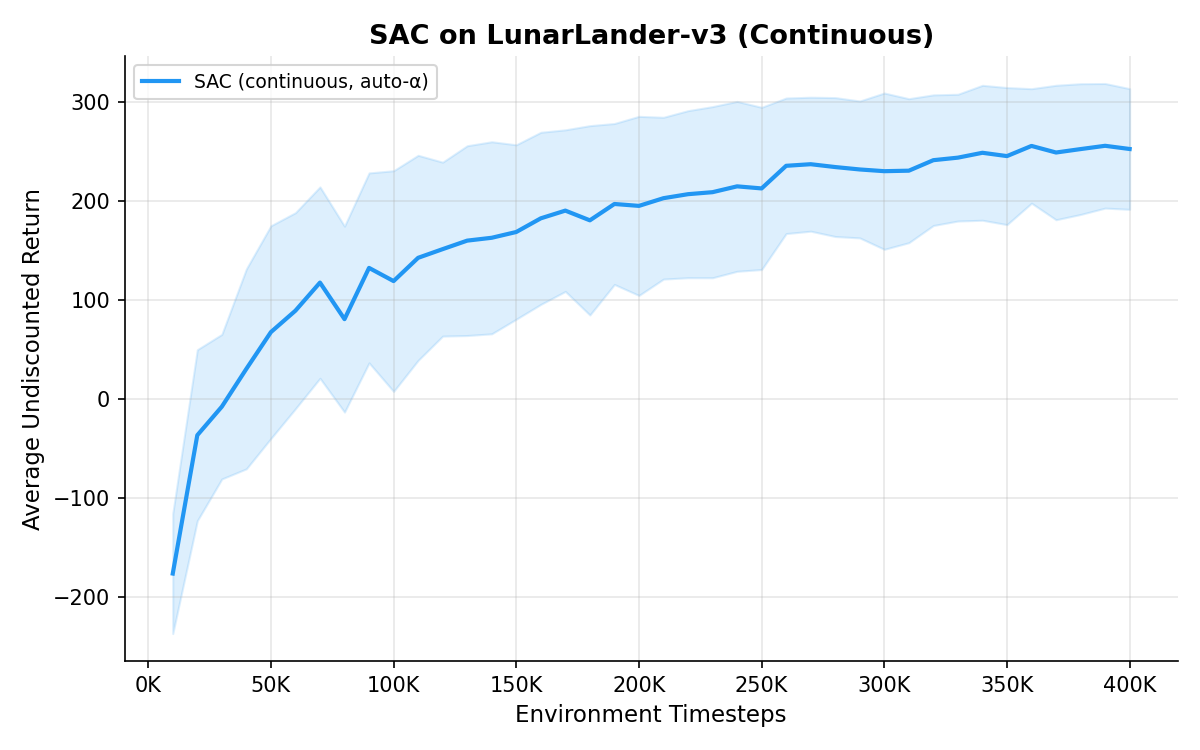
\includegraphics[width=0.7\textwidth]{images/ll_sac_continuous.png}
        \caption{SAC (auto-$\alpha$) on continuous LunarLander-v3, mean $\pm$ std over 15 seeds. Return rises from $\sim$$-180$ to $\sim$$+250$ in $\sim$400K steps.}
        \label{fig:ll_sac_cont}
    \end{figure}

    \item \textbf{Behaviour across training stages.} Reading Figure~\ref{fig:ll_sac_cont} together with rollout videos of intermediate checkpoints, three qualitatively distinct regimes are visible.
    \begin{itemize}
        \item \emph{Initial ($0$--$30$K steps, return $\approx -180$):} the policy is essentially the random warm-up policy followed by a near-uniform tanh-Gaussian. The lander fires the main and side engines at random, immediately tips over and crashes, so the $-100$ crash penalty plus accumulated shaping costs dominate.
        \item \emph{Intermediate-I ``don't crash'' ($\sim$30K--100K, return $\approx 0$--$100$):} the agent learns the cheapest way to stop losing reward, which is to \emph{avoid crashing} rather than to land. Two sub-optima are observed in this band: (a) a \textbf{hover/float} policy where the lander throttles the main engine continuously to stay aloft, trading the $-0.3$/step fuel cost against the $-100$ crash penalty, and (b) a \textbf{drift-out-of-bounds} policy where the lander tips sideways until the episode terminates with no big bonus or penalty. The mean curve flattens near $0$ for $\sim$30K--60K steps -- this plateau is the signature of these two local optima.
        \item \emph{Intermediate-II ``soft touchdown, wrong spot'' ($\sim$100K--250K, return $\approx 100$--$200$):} entropy still encourages exploration, and the agent discovers that turning off the main engine near the ground is profitable. It now manages soft landings but often outside the flag pads, collecting the descent shaping but missing the $+100$ landing bonus. Variance across seeds is large here ($\sigma\approx 100$), reflecting different seeds settling on different ``land-anywhere'' policies.
        \item \emph{Final ($\sim$300K--400K, return $\approx 240$--$260$):} $\alpha$ has decayed (automated tuning lowers it as the policy becomes confident), and the policy converges to the near-optimal behaviour: lateral thrust to centre over the pad, controlled vertical descent with throttled main engine, both legs touching down simultaneously between the flags. Returns settle into the ``solved'' band ($>200$) with shrinking variance.
    \end{itemize}
    Yes, there are clear intermediate local optima: the hover/float policy and the land-anywhere policy. Both are entropy-stable basins because escaping them requires a coordinated sequence (descend \emph{and} centre \emph{and} kill velocity) that random exploration rarely strings together; SAC eventually escapes them only because the maximum-entropy objective keeps the policy stochastic enough to occasionally stumble onto the pad.

    \item \textbf{Hover-reward environment and reward switch ($+200\rightarrow -100$).} We add a one-shot $+200$ bonus the first time the lander enters the hover box ($|x|<0.1$, $0.4<|y|<0.6$), train for $250$K steps, then flip the bonus to $-100$ and continue training to $500$K steps. Two SAC variants are compared: \textbf{fixed} $\alpha=0.01$ and \textbf{auto} $\alpha$ (target entropy $-2$). Figure~\ref{fig:ll_hover} shows the learning curves; the dashed line marks the reward switch.

    \begin{figure}[H]
        \centering
        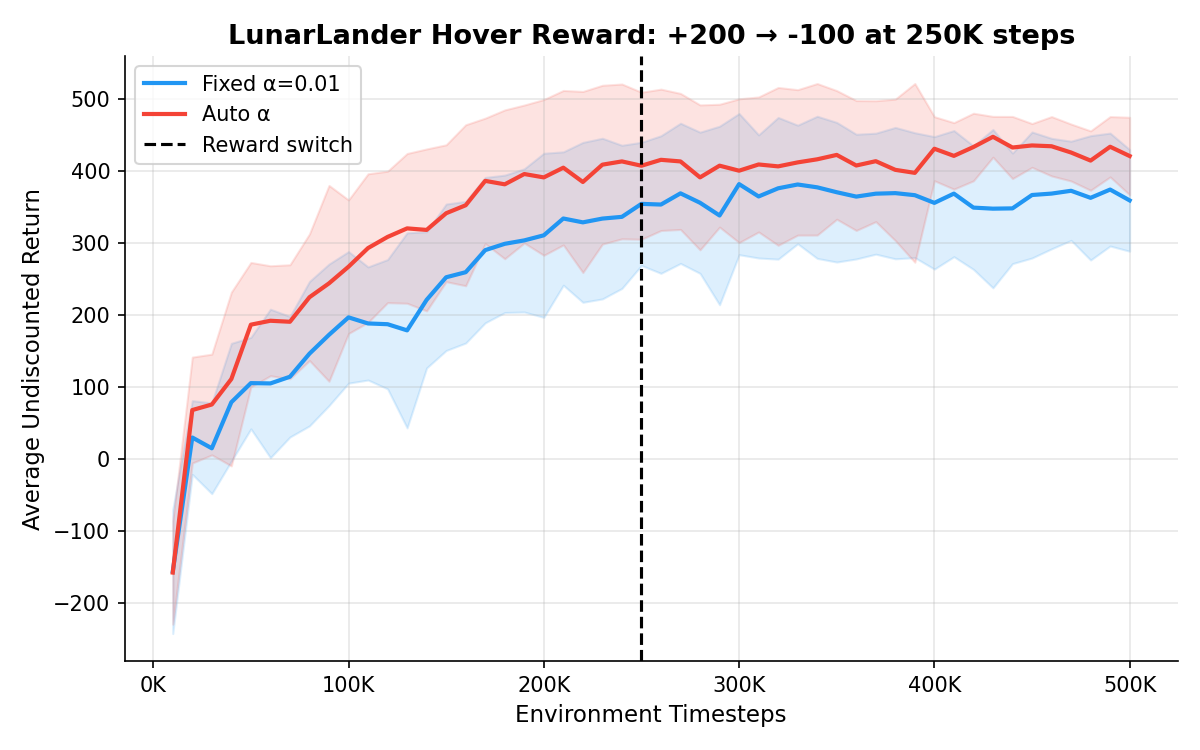
\includegraphics[width=0.7\textwidth]{images/ll_hover_comparison.png}
        \caption{LunarLander with hover bonus, switching from $+200$ to $-100$ at $250$K steps (dashed line). Auto-$\alpha$ (red) vs.\ fixed $\alpha=0.01$ (blue), mean $\pm$ std over 15 seeds.}
        \label{fig:ll_hover}
    \end{figure}

    \begin{enumerate}[label=(\alph*)]
        \item \textbf{Quantitative + qualitative comparison.}
        \emph{Before the switch ($0$--$250$K, hover $= +200$).} Both variants learn to claim the hover bonus and to land, but auto-$\alpha$ is uniformly faster and higher: it reaches $\approx 270$ by $100$K and plateaus near $\approx 410$ by $250$K, while fixed $\alpha=0.01$ trails by roughly $50$--$80$ return (reaching only $\approx 197$ at $100$K and $\approx 355$ at $250$K). Qualitatively both policies pass through the hover box on the way down and then land between the flags, harvesting both the $+200$ hover bonus and the $+100$ landing bonus.

        \emph{After the switch ($250$K--$500$K, hover $= -100$).} The expected optimal behaviour changes: a competent agent should now \emph{avoid} the hover box and still land. The auto-$\alpha$ curve briefly dips around the switch but then climbs and stabilises around $\approx 430$ -- in fact \emph{higher} than its pre-switch value, because the policy has actually re-routed around the box and so collects neither the $-100$ nor the $+200$, while keeping the $+100$ landing bonus and improved shaping. The fixed-$\alpha$ curve, in contrast, stays essentially flat at $\approx 360$--$380$ from the switch onward and never recovers the auto-$\alpha$ level. Inspecting rollouts, the fixed-$\alpha$ policy keeps flying through the same trajectory it learned in phase~1 and pays the $-100$ on roughly every episode, whereas the auto-$\alpha$ policy learns to deflect laterally just above the hover box before descending.

        The qualitative gap is exactly what one would predict from the entropy: at $\alpha=0.01$ the policy has already collapsed to a near-deterministic ``go-through-the-box'' trajectory by $250$K and there is essentially no exploration left to discover the alternative deflected path; under auto-$\alpha$ the temperature is automatically re-raised when the post-switch returns drop, exploration is restored, and the policy can reorganise around the new reward landscape.

        \item \textbf{What this says about the maximum-entropy formulation of SAC.}
        The experiment cleanly illustrates the role of the entropy bonus. Under a \emph{fixed} small $\alpha$ the entropy term is essentially decorative once the policy converges: the stochasticity collapses, and any change in the environment that requires a structurally new trajectory cannot be discovered -- the agent is stuck with whatever it learned first. Under \emph{automated} temperature tuning, $\alpha$ is the dual variable of the target-entropy constraint, so when the post-switch returns drop and the policy becomes overconfident relative to the new optimum, the dual variable is automatically driven up, the policy re-randomises, and the agent rediscovers a better mode.

        In short, the maximum-entropy framework is not just an exploration heuristic for the start of training; it is the mechanism that gives SAC its robustness to \emph{non-stationary} rewards. The temperature is the knob that controls the trade-off between commitment to the current policy and openness to new ones, and tying it to a target-entropy constraint (rather than fixing it) makes the algorithm adapt that knob automatically as the task changes scale or shape. This is also why fixed-$\alpha$ SAC is fragile to reward re-scaling (cf.\ Problem 1.5b): the ``right'' $\alpha$ is a function of the current reward magnitude, and automated tuning is what keeps the entropy contribution commensurate with the reward signal at every stage of training.
    \end{enumerate}

    \item \textbf{Discrete-action LunarLander.}
    \begin{enumerate}[label=(\alph*)]
        \item \textbf{Discrete SAC.} For a discrete action space $\mathcal{A}=\{1,\ldots,|\mathcal{A}|\}$ the policy is a categorical distribution $\pi_\phi(\cdot\mid s)$ with $|\mathcal{A}|$ logits, so the integrals over actions in the standard SAC updates collapse into exact sums and the re-parameterization trick is no longer needed. Concretely:
        \begin{itemize}
            \item \emph{Critic:} each $Q_{\theta_i}(s)$ now outputs a vector of $|\mathcal{A}|$ values. The soft target uses the expectation under the next-state policy: \\
            \[
              y = r + \gamma \sum_{a'} \pi_{\phi}(a'\mid s')\Big[\min_i Q_{\bar\theta_i}(s', a') - \alpha \log \pi_\phi(a'\mid s')\Big].
            \]
            \item \emph{Actor:} the policy loss is the expectation (not a sample) of $\alpha\log\pi - \min_i Q_i$ under $\pi$: \\
            \[
              \mathcal{L}_\pi = \mathbb{E}_{s}\!\sum_a \pi_\phi(a\mid s)\big[\alpha\log\pi_\phi(a\mid s) - \min_i Q_{\theta_i}(s,a)\big].
            \]
            \item \emph{Temperature:} target entropy is set to $\bar{\mathcal{H}} = 0.98\cdot(-\log(1/|\mathcal{A}|))$, i.e.\ a fraction of the maximum entropy of the categorical, and $\alpha$ is updated with the same dual-gradient rule as continuous SAC.
        \end{itemize}
        Everything else (replay buffer, target networks with Polyak averaging, clipped double-Q, $\gamma=0.99$, Adam, $10$K random warm-up) is identical to the continuous version.

        \item \textbf{Discrete-SAC results on LunarLander-v3 (discrete).} Trained for $500$K steps with $15$ seeds and the same evaluation protocol as the continuous case (20 offline episodes every $10$K steps). Figure~\ref{fig:ll_discrete} (blue) shows the mean $\pm 1$ std curve. Discrete-SAC starts at $\approx -660$, crosses zero by $\sim$50K, plateaus near $\sim$70 until $\sim$200K (the same ``avoid-crashing'' local optimum seen in the continuous case), and only escapes to the solved band ($\geq 200$) toward the end of training, finishing at $\approx 200 \pm 101$.

        \begin{figure}[H]
            \centering
            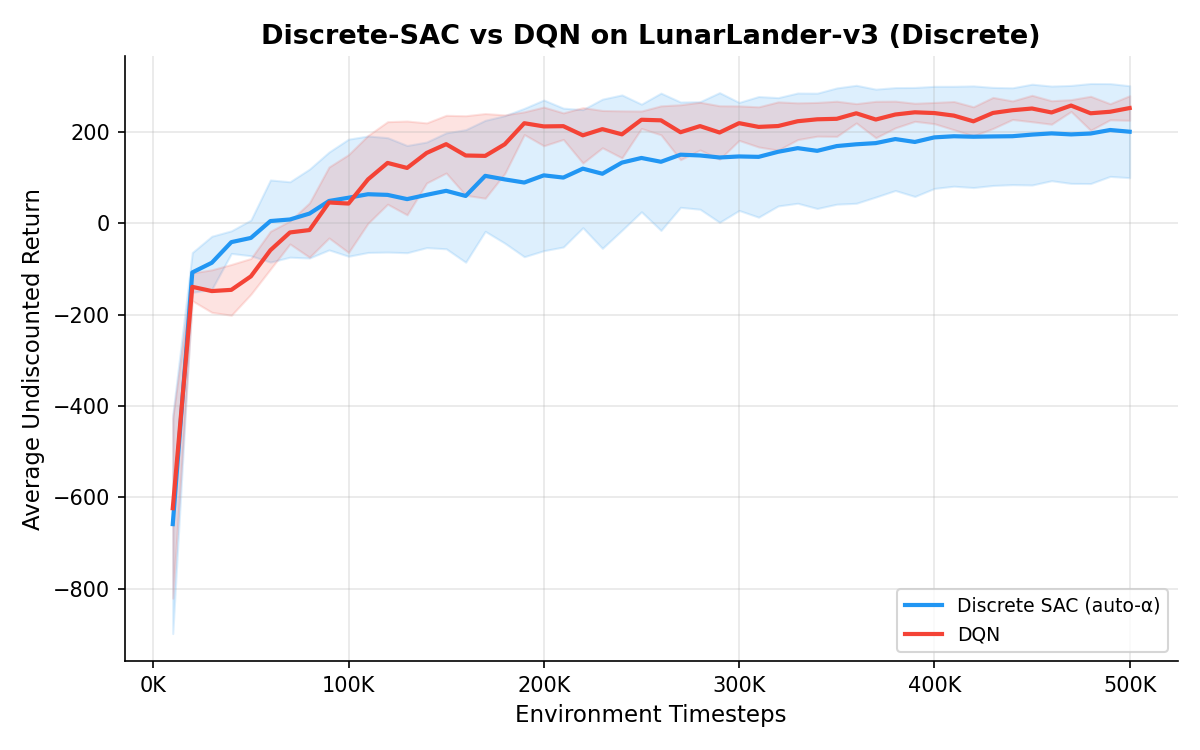
\includegraphics[width=0.7\textwidth]{images/ll_discrete_sac_vs_dqn.png}
            \caption{Discrete-SAC (auto-$\alpha$, blue) vs DQN (red) on discrete LunarLander-v3, mean $\pm$ std over 15 seeds.}
            \label{fig:ll_discrete}
        \end{figure}

        \item \textbf{Comparison with DQN.} DQN is trained on the same environment for $500$K steps with $15$ seeds. From Figure~\ref{fig:ll_discrete}, DQN reaches the ``solved'' band ($\geq 200$) by $\sim$200K steps and finishes at $\approx 252 \pm 27$, whereas discrete-SAC ends at $\approx 200 \pm 101$. DQN is therefore both faster (sample-efficient) \emph{and} much lower variance across seeds in this environment; discrete-SAC eventually approaches DQN's level but several seeds still sit well below the solved threshold at $500$K, which inflates its standard deviation.

        \item \textbf{Which to prefer for discrete actions?}
        For this environment, and discrete-action tasks in general, we would prefer \textbf{DQN}, based on the two criteria asked:
        \begin{itemize}
            \item \emph{Performance and sample efficiency:} DQN learns faster and to a tighter, higher final return on LunarLander-discrete. The maximum-entropy objective of SAC, which is genuinely useful in continuous action spaces (where exploration is hard and the policy's stochasticity matters), buys less in a small $4$-action discrete setting -- $\epsilon$-greedy plus the natural noise of a value-based bootstrap is already enough exploration, and the extra actor network and entropy machinery just adds variance.
            \item \emph{Ease of implementation:} DQN is a single $Q$-network with a target copy, an $\epsilon$-greedy policy and a $1$-line Bellman target. Discrete-SAC needs two critics, a separate categorical actor, exact expectations over actions in both the actor and the critic update, and a learnable temperature with target entropy chosen as a fraction of $\log|\mathcal{A}|$. That is strictly more code, more hyperparameters, and more places to bug.
        \end{itemize}
        Discrete-SAC is still a reasonable choice when (i) the action space is large enough that $\epsilon$-greedy exploration is too crude, or (ii) one wants the same algorithmic recipe to apply uniformly to both continuous and discrete tasks. Outside those cases, DQN (or a Rainbow-style refinement) is simpler, faster to tune, and -- as Figure~\ref{fig:ll_discrete} shows -- empirically better on this environment.
    \end{enumerate}
\end{enumerate}

% ── Q3: Reacher ─────────────────────────────────────────────────────────────
\paragraph*{Problem 3}
\begin{enumerate}
    \item \textbf{SAC implementation on Reacher for $\mathcal{R}_a, \mathcal{R}_b, \mathcal{R}_c$.}
    We implement SAC (clipped double-Q, squashed Gaussian policy with re-parameterization, $\gamma=0.99$, $10$K random-action warm-up) with automated temperature tuning using target entropy $\bar{\mathcal{H}}=-\dim(\mathcal{A})$. The same agent is trained separately under each reward formulation for $5\times10^5$ environment steps. Every $10$K steps we evaluate the current policy with $20$ offline episodes and log returns under \emph{all} three reward functions $\mathcal{R}_a,\mathcal{R}_b,\mathcal{R}_c$ simultaneously, so that cross-evaluation curves can be obtained from a single training run per reward.

    \item \textbf{Self-evaluation curves: SAC-$\mathcal{R}_i$ evaluated against $\mathcal{R}_i$.}
    Figures~\ref{fig:self_a}, \ref{fig:self_b}, \ref{fig:self_c} show the average un-discounted return (mean $\pm$ std over $15$ seeds) of SAC-$\mathcal{R}_i$ measured under its own training reward.

    \begin{figure}[h]
        \centering
        \begin{minipage}{0.32\textwidth}
            
\includegraphics[width=\linewidth]{images/fig_A_self_eval_rra.png}
            \caption{SAC-$\mathcal{R}_a$ on $\mathcal{R}_a$.}\label{fig:self_a}
        \end{minipage}\hfill
        \begin{minipage}{0.32\textwidth}
            
\includegraphics[width=\linewidth]{images/fig_A_self_eval_rrb.png}
            \caption{SAC-$\mathcal{R}_b$ on $\mathcal{R}_b$.}\label{fig:self_b}
        \end{minipage}\hfill
        \begin{minipage}{0.32\textwidth}
            
\includegraphics[width=\linewidth]{images/fig_A_self_eval_rrc.png}
            \caption{SAC-$\mathcal{R}_c$ on $\mathcal{R}_c$.}\label{fig:self_c}
        \end{minipage}
    \end{figure}

    \textbf{Learning speed:} SAC-$\mathcal{R}_a$ and SAC-$\mathcal{R}_b$ both converge rapidly: returns rise sharply within the first $\sim$100K steps and plateau near $\sim$880--950 by $\sim$200K steps. SAC-$\mathcal{R}_c$ is dramatically slower; even after $5\times10^5$ steps it has not converged and still has return $\approx -330$ with very wide confidence bands.

    \textbf{Why?} $\mathcal{R}_b$ is a dense $\{0,1\}$ in-target indicator -- every step the agent gets immediate, informative feedback, so credit assignment is easy and learning is fast. $\mathcal{R}_a$ adds a shaping term ($-\|x_{\text{goal}}-x_{\text{pos}}\|-\|\text{action}\|^2$) that gives a smooth gradient toward the target even when the arm is far away, so it is roughly as fast as $\mathcal{R}_b$ (sometimes a hair slower because of the action penalty creating a small conservatism bias). $\mathcal{R}_c$ gives a constant $-1$ until termination -- this is essentially a sparse, terminal-only signal: the agent only learns by occasionally stumbling into the goal and being terminated, and the timeout penalty kicks in only at $T=1000$. With long horizons and a near-constant reward, the gradient signal early in training is extremely weak, which explains the slow, high-variance learning curve.

    \item \textbf{Does the learned policy actually achieve the desired behaviour?}
    \begin{enumerate}[label=(\alph*)]
        \item \textbf{Steps-to-goal and steps-in-target ($500$ episodes $\times$ $5000$ steps).}
        Figure~\ref{fig:bar} reports the two metrics for the final policy under each reward formulation.

        \begin{figure}[h]
            \centering
            
\includegraphics[width=0.85\textwidth]{images/fig_B_bar_chart.png}
            \caption{Steps to first reach target (left, lower is better) and steps spent inside the target (right, higher is better) for the final SAC-$\mathcal{R}_i$ policies, $500$ episodes of length $5000$.}
            \label{fig:bar}
        \end{figure}

        Numerically, SAC-$\mathcal{R}_a$ reaches the target in $\approx 142$ steps and remains in it for $\approx 925$ of the next $\sim4858$ steps; SAC-$\mathcal{R}_b$ reaches it slightly faster ($\approx 119$ steps) and stays slightly longer ($\approx 945$); SAC-$\mathcal{R}_c$ reaches the target only in $\approx 975$ steps on average and stays for only $\approx 38$ steps.

        \item \textbf{Which reward best achieves the desired behaviour?}
        $\mathcal{R}_b$ does, very closely followed by $\mathcal{R}_a$. Both produce policies that reach the target quickly ($\sim$120--140 steps) and \emph{remain} in it for the vast majority of the remaining horizon (the cap on ``steps in target'' is constrained only by the time taken to first arrive). $\mathcal{R}_c$ fails the desired behaviour on \emph{both} axes: it neither reaches the target quickly nor stays there. The reason is structural: $\mathcal{R}_c$ terminates the episode the moment the arm enters the target with near-zero velocity, so the agent is never rewarded for \emph{remaining} -- once it has learned to terminate, there is no incentive to stay. Combined with the timeout reset penalty being its only non-constant signal during training, the resulting policy under $5000$-step evaluation (where termination is disabled / the same policy is rolled out continuously) drifts out of the target almost immediately. $\mathcal{R}_a$ adds an action-norm penalty on top of distance shaping, which slightly pushes the arm to approach more conservatively than $\mathcal{R}_b$, hence its marginally larger steps-to-goal; but both are essentially solving the task.

        \item \textbf{Cross-evaluation: SAC-$\mathcal{R}_j$ measured under $\mathcal{R}_i$ for all $(i,j)$.}
        Figures~\ref{fig:cross_a}, \ref{fig:cross_b}, \ref{fig:cross_c} show every SAC agent evaluated under each of the three rewards.

        \begin{figure}[h]
            \centering
            \begin{minipage}{0.32\textwidth}
                
\includegraphics[width=\linewidth]{images/fig_C_cross_eval_against_rra.png}
                \caption{Eval under $\mathcal{R}pl_a$.}\label{fig:cross_a}
            \end{minipage}\hfill
            \begin{minipage}{0.32\textwidth}
                
\includegraphics[width=\linewidth]{images/fig_C_cross_eval_against_rrb.png}
                \caption{Eval under $\mathcal{R}_b$.}\label{fig:cross_b}
            \end{minipage}\hfill
            \begin{minipage}{0.32\textwidth}
                
\includegraphics[width=\linewidth]{images/fig_C_cross_eval_against_rrc.png}
                \caption{Eval under $\mathcal{R}_c$.}\label{fig:cross_c}
            \end{minipage}
        \end{figure}

        \begin{enumerate}[label=(\roman*)]
            \item \textbf{Per-plot analysis.}
            \emph{Evaluated on $\mathcal{R}_a$:} SAC-$\mathcal{R}_a$ and SAC-$\mathcal{R}_b$ are essentially overlapping ($\approx 880$--$900$); SAC-$\mathcal{R}_c$ trails far behind ($\approx 600$ at the end, still rising).
            \emph{Evaluated on $\mathcal{R}_b$:} again SAC-$\mathcal{R}_a$ and SAC-$\mathcal{R}_b$ overlap ($\approx 940$); SAC-$\mathcal{R}_c$ reaches only $\approx 700$.
            \emph{Evaluated on $\mathcal{R}_c$:} SAC-$\mathcal{R}_a$ and SAC-$\mathcal{R}_b$ converge to $\approx -180$ within $\sim$200K steps and \emph{outperform} SAC-$\mathcal{R}_c$ itself ($\approx -330$ at $5\times10^5$ steps), which is the agent that was trained on this very signal.
            Across all three plots, SAC-$\mathcal{R}_a$ and SAC-$\mathcal{R}_b$ are nearly indistinguishable in both speed and final value; SAC-$\mathcal{R}_c$ is consistently the slowest and worst, including under its own metric.

            \item \textbf{Cases where SAC-$\mathcal{R}_j$ beats SAC-$\mathcal{R}_i$ ($j\neq i$).}
            Yes. Most strikingly, SAC-$\mathcal{R}_a$ and SAC-$\mathcal{R}_b$ both \emph{outperform} SAC-$\mathcal{R}_c$ when evaluated on $\mathcal{R}_c$ itself. This means a policy trained on a denser reward generalizes to the sparse metric better than one trained directly on the sparse metric. Structurally: $\mathcal{R}_a$ and $\mathcal{R}_b$ provide a strong gradient that drives the arm into the target quickly; once there, the policy stays, which under $\mathcal{R}_c$ corresponds to fewer accumulated $-1$'s and (with our termination/penalty implementation) a higher return. Conversely, SAC-$\mathcal{R}_c$ can only learn to reach the target by chance and never receives positive reinforcement for the ``stay'' part of the task -- it is exactly the credit-assignment failure that sparse, time-only rewards are known for. The result indicates that good behavior is much more determined by reward density and shaping than by whether the reward exactly matches the evaluation metric: a denser surrogate is a better optimization target than the true sparse objective.

            \item \textbf{Overall Rating:}
            \begin{itemize}
                \item \emph{Ease of specification:} $\mathcal{R}_c$ is easiest (just $-1$ everywhere) and $\mathcal{R}_b$ a close second (binary indicator); $\mathcal{R}_a$ requires picking distance and action-norm scales.
                \item \emph{Learning efficiency:} $\mathcal{R}_b\approx \mathcal{R}_a \gg \mathcal{R}_c$. Dense feedback wins by a large margin.
                \item \emph{Achievement of the desired behaviour:} $\mathcal{R}_b$ best (fastest reach, longest stay), $\mathcal{R}_a$ a very close second, $\mathcal{R}_c$ fails both criteria.
            \end{itemize}
            \textbf{Recommendation:} use $\mathcal{R}_b$ in practice. It is almost as easy to specify as $\mathcal{R}_c$, learns as fast as the shaped $\mathcal{R}_a$, and produces the best ``reach-and-stay'' behaviour without requiring tuning of distance/action-norm scales. $\mathcal{R}_a$ is a reasonable alternative when one wants to additionally regularize action magnitudes. $\mathcal{R}_c$ is not recommended: it is slow to learn, terminates on first contact (so never teaches ``stay''), and is dominated even on its own metric by agents trained with denser rewards.
        \end{enumerate}
    \end{enumerate}
\end{enumerate}

\paragraph*{Problem 4 (Bonus)}
\begin{enumerate}
    \item \textbf{PEBBLE on Pendulum vs.\ SAC trained on the ground-truth reward.}
    PEBBLE replaces the ground-truth reward by a \emph{learned} reward $\hat r_\psi(s,a)$ that is trained from pairwise preferences between trajectory segments. Concretely, every $2{,}000$ environment steps we sample $n_{\text{query}}=5$ random pairs of length-$50$ segments $(\sigma^1,\sigma^2)$ from the replay, query a simulated teacher that knows the ground-truth (GT) reward, and record the preference label
    \[
        y(\sigma^1,\sigma^2) = \mathbb{1}\!\left[\textstyle\sum_t r^{\text{gt}}(\sigma^1_t) > \sum_t r^{\text{gt}}(\sigma^2_t)\right].
    \]
    The reward network is updated by minimising the Bradley--Terry cross-entropy loss on the preference buffer:
    \[
      \mathcal{L}_{\text{reward}}(\psi) \;=\; -\!\!\!\sum_{(\sigma^1,\sigma^2,y)\in\mathcal{D}_{\text{pref}}}\!\!\Big[\, y\log P_\psi[\sigma^1\!\succ\!\sigma^2] + (1-y)\log P_\psi[\sigma^2\!\succ\!\sigma^1]\,\Big],
    \]
    \[
      P_\psi[\sigma^1\!\succ\!\sigma^2] \;=\; \frac{\exp\!\sum_t \hat r_\psi(\sigma^1_t)}{\exp\!\sum_t \hat r_\psi(\sigma^1_t) + \exp\!\sum_t \hat r_\psi(\sigma^2_t)}.
    \]
    SAC is run on top of this learned reward, with the entire replay buffer being \emph{relabelled} by $\hat r_\psi$ after every reward update so the critic is always consistent with the current $\psi$. We follow PEBBLE's prescription of an unsupervised pre-training phase: for the first $10$K steps the agent explores with a state-entropy intrinsic reward, then preference queries begin.

    We compare PEBBLE (budget $=500$, which in practice schedules $5$ queries every $2$K steps and converges to $\approx 200$ realised queries over $100$K steps -- the rest of the budget is never spent because the trainer caps at one batch per session) against \textbf{SAC trained on the GT reward}. Both algorithms run for $100$K steps on the modified Pendulum-v1 with $\theta_{\text{target}}\in\{0,-60,90,120,-150\}$, $15$ seeds each, evaluated by $20$ offline episodes every $10$K steps and reported in \emph{ground-truth} return.

    \begin{figure}[H]
        \centering
        \begin{minipage}{0.32\textwidth}
            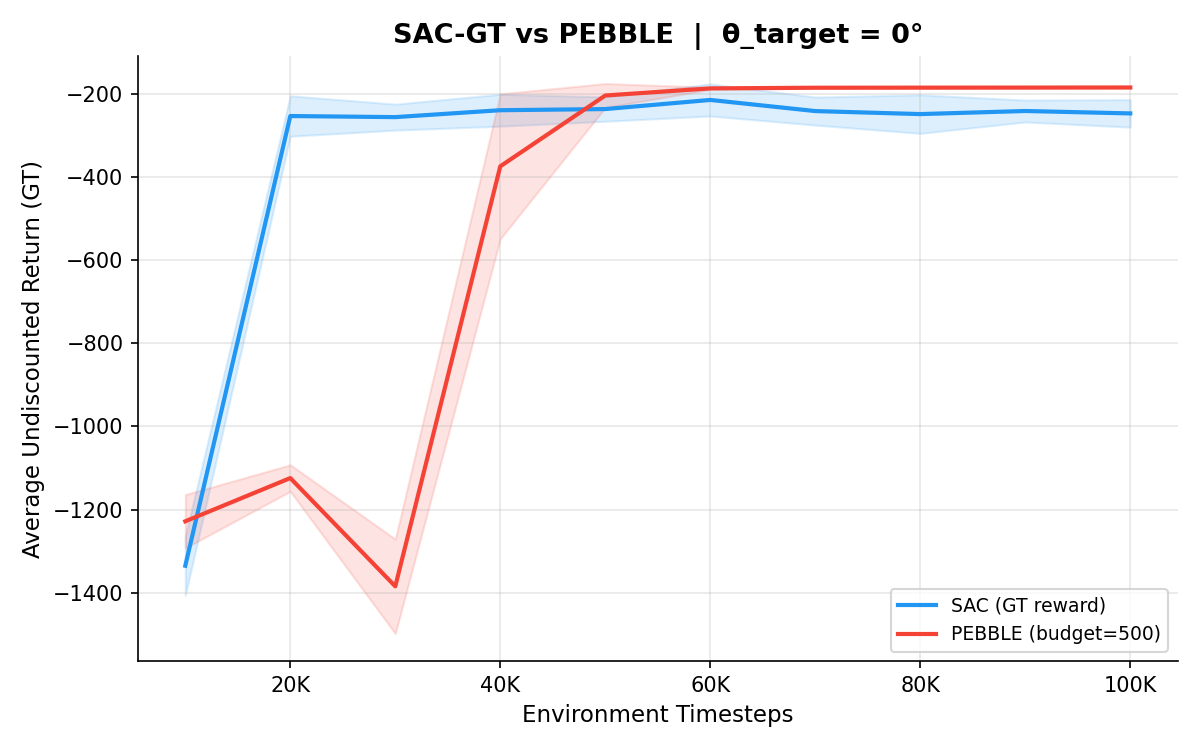
\includegraphics[width=\linewidth]{images/pebble_sac_vs_pebble_theta0.png}
            \caption*{$\theta_{\text{target}}=0^\circ$}
        \end{minipage}\hfill
        \begin{minipage}{0.32\textwidth}
            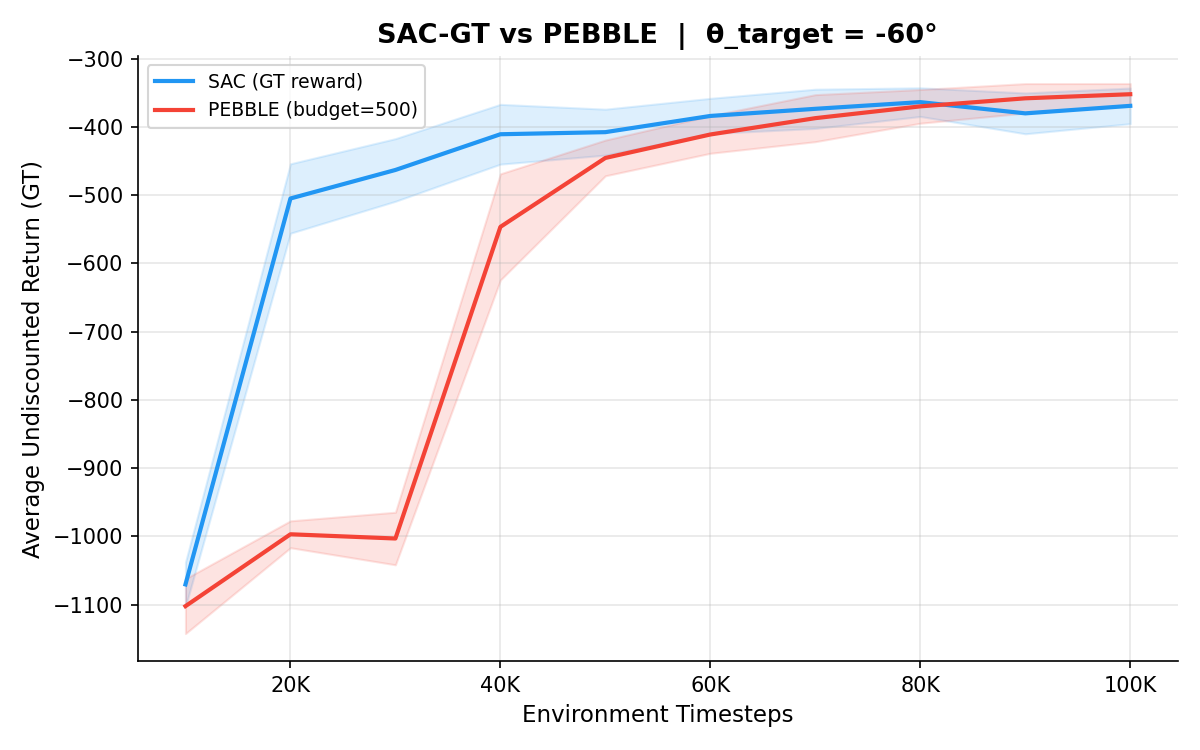
\includegraphics[width=\linewidth]{images/pebble_sac_vs_pebble_theta-60.png}
            \caption*{$\theta_{\text{target}}=-60^\circ$}
        \end{minipage}\hfill
        \begin{minipage}{0.32\textwidth}
            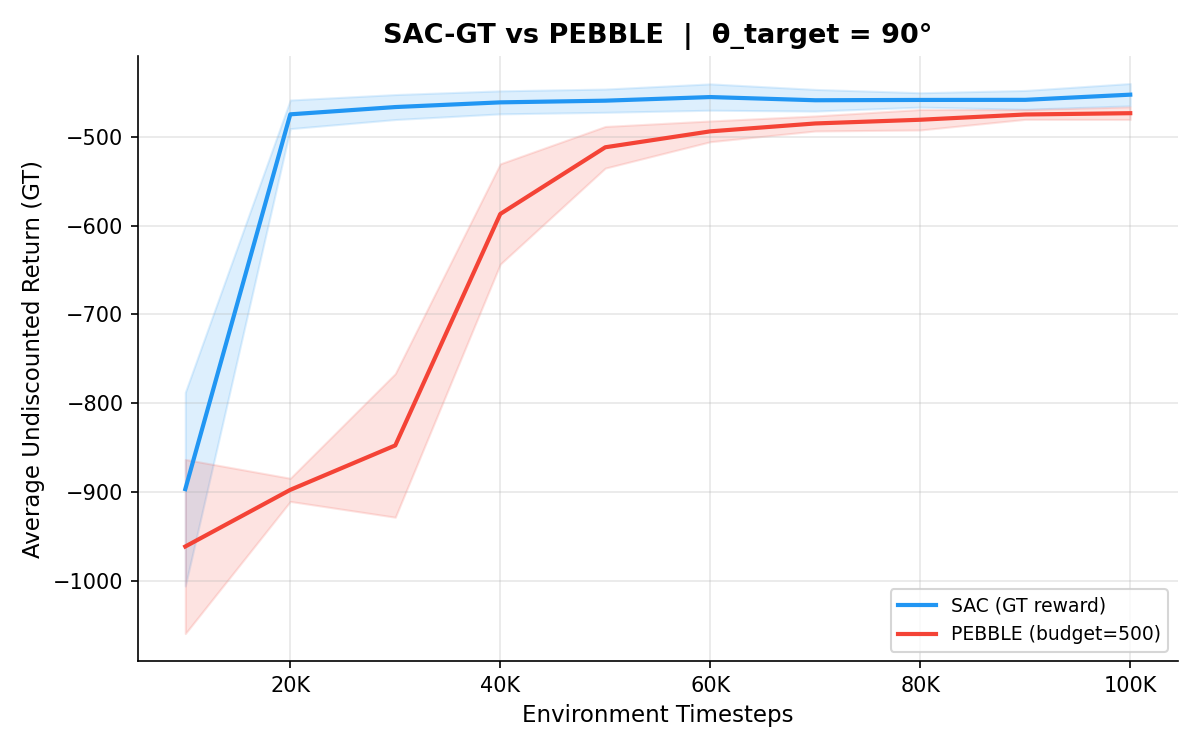
\includegraphics[width=\linewidth]{images/pebble_sac_vs_pebble_theta90.png}
            \caption*{$\theta_{\text{target}}=90^\circ$}
        \end{minipage}\\[4pt]
        \begin{minipage}{0.32\textwidth}
            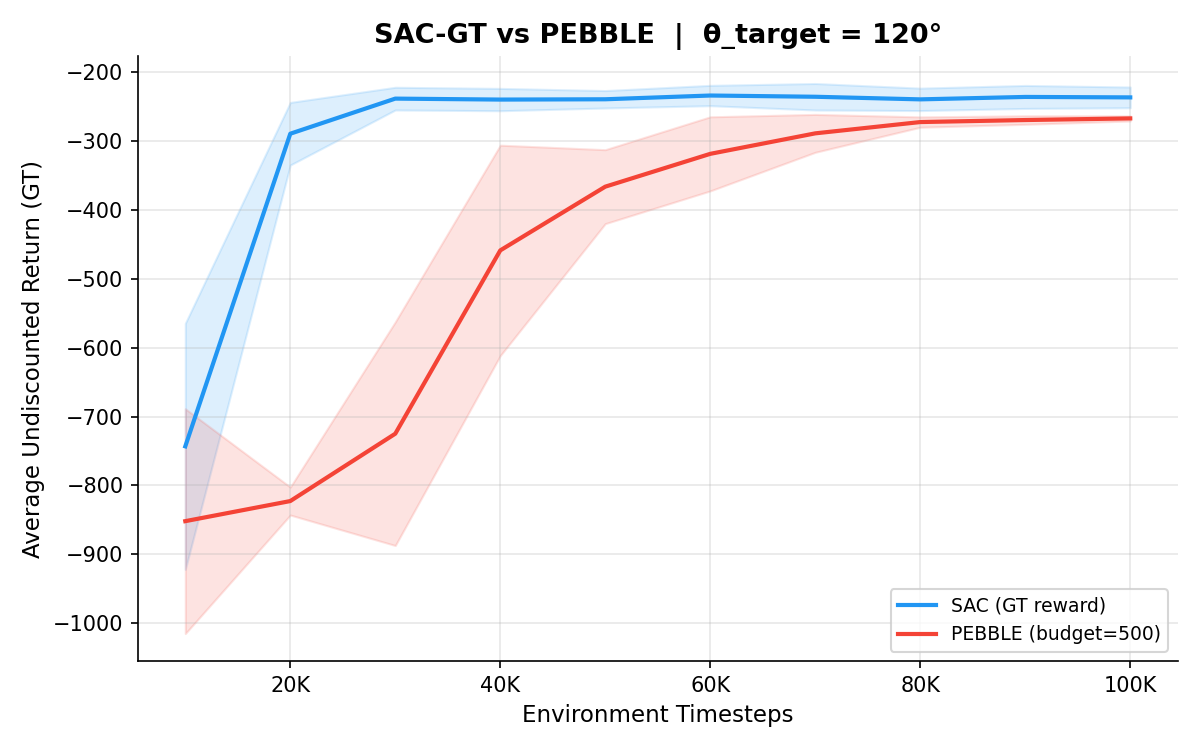
\includegraphics[width=\linewidth]{images/pebble_sac_vs_pebble_theta120.png}
            \caption*{$\theta_{\text{target}}=120^\circ$}
        \end{minipage}\hfill
        \begin{minipage}{0.32\textwidth}
            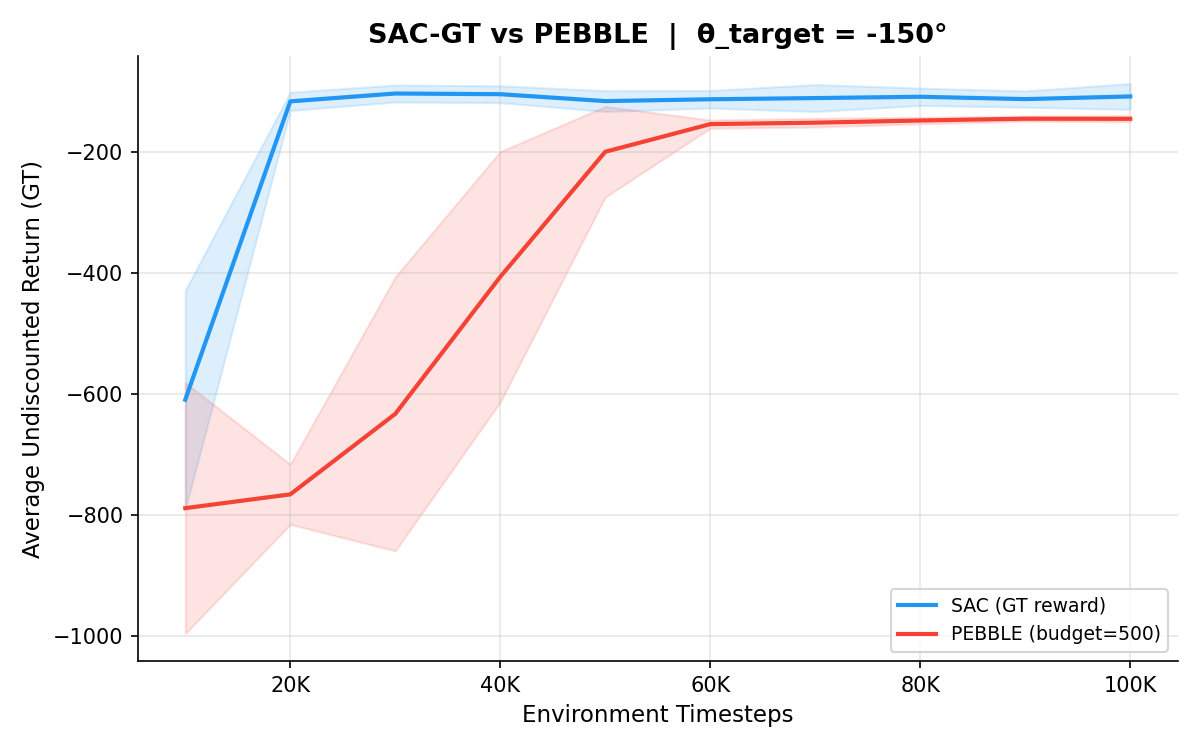
\includegraphics[width=\linewidth]{images/pebble_sac_vs_pebble_theta-150.png}
            \caption*{$\theta_{\text{target}}=-150^\circ$}
        \end{minipage}\hfill
        \begin{minipage}{0.32\textwidth}\centering\vfill (mean $\pm$ std, $15$ seeds; budget $=500$, only $\approx 200$ queries actually used)\vfill\end{minipage}
        \caption{SAC trained on the ground-truth reward (blue) vs PEBBLE (red, budget $500$) on Pendulum-v1 with five different target angles.}
        \label{fig:pebble_vs_sac}
    \end{figure}

    \textbf{Learning efficiency.} Across all five targets, SAC-GT crosses the steep early descent within $\approx 20$K steps (its first useful evaluation point), whereas PEBBLE remains essentially flat at its initial return until $\approx 30$--$40$K steps and only then starts to climb. The lag is structurally inevitable: PEBBLE first spends $10$K steps in the unsupervised pre-train phase and then a further $\sim$10--20K steps in collecting enough preference labels and fitting $\hat r_\psi$ before the learned reward provides useful gradient. So PEBBLE is roughly $20$--$30$K env-steps slower to take off than SAC-GT at every target.

    \textbf{Final performance.} Once PEBBLE catches up, it tracks SAC-GT remarkably closely:
    \begin{itemize}
        \item $\theta=0^\circ$: SAC-GT $\approx -247\pm33$, PEBBLE $\approx -184\pm1$ -- \emph{PEBBLE actually finishes higher} (the learned reward has lower seed-variance than the noisy quadratic GT reward and converges to a tighter steady-state policy).
        \item $\theta=-60^\circ$: SAC-GT $\approx -369\pm26$, PEBBLE $\approx -352\pm16$ -- essentially identical.
        \item $\theta=90^\circ$: SAC-GT $\approx -453\pm13$, PEBBLE $\approx -473\pm7$ -- PEBBLE within $\sim 20$ return of GT on the hardest target.
        \item $\theta=120^\circ$: SAC-GT $\approx -236\pm15$, PEBBLE $\approx -267\pm4$ -- gap of $\sim 30$.
        \item $\theta=-150^\circ$: SAC-GT $\approx -109\pm21$, PEBBLE $\approx -146\pm5$ -- gap of $\sim 37$, but PEBBLE is much lower-variance.
    \end{itemize}
    Overall PEBBLE matches SAC-GT to within $\sim 5$--$15\%$ of the final return on every target despite using $\sim 200$ preference labels in place of an explicit reward function -- and on the easiest stable target ($\theta=0$) it even slightly outperforms SAC-GT. The trade-off is exactly the one PEBBLE was designed to expose: a one-time $\sim$20K-step warm-up cost in sample efficiency in exchange for never having to design or hand-shape a reward.

    \item \textbf{Feedback-budget ablation.} We sweep the maximum allowed preference queries $B\in\{50,100,200,500,1000\}$ for the same five targets ($15$ seeds each, $100$K steps). The actual number of queries the trainer issues is capped by its schedule ($5$ queries every $2$K steps starting after the $10$K-step warm-up), so budgets $\geq 200$ all realise the \emph{same} $\sim 200$ queries; only $B\in\{50,100\}$ are genuinely query-limited. Curves are reported in ground-truth return.

    \begin{figure}[H]
        \centering
        \begin{minipage}{0.32\textwidth}
            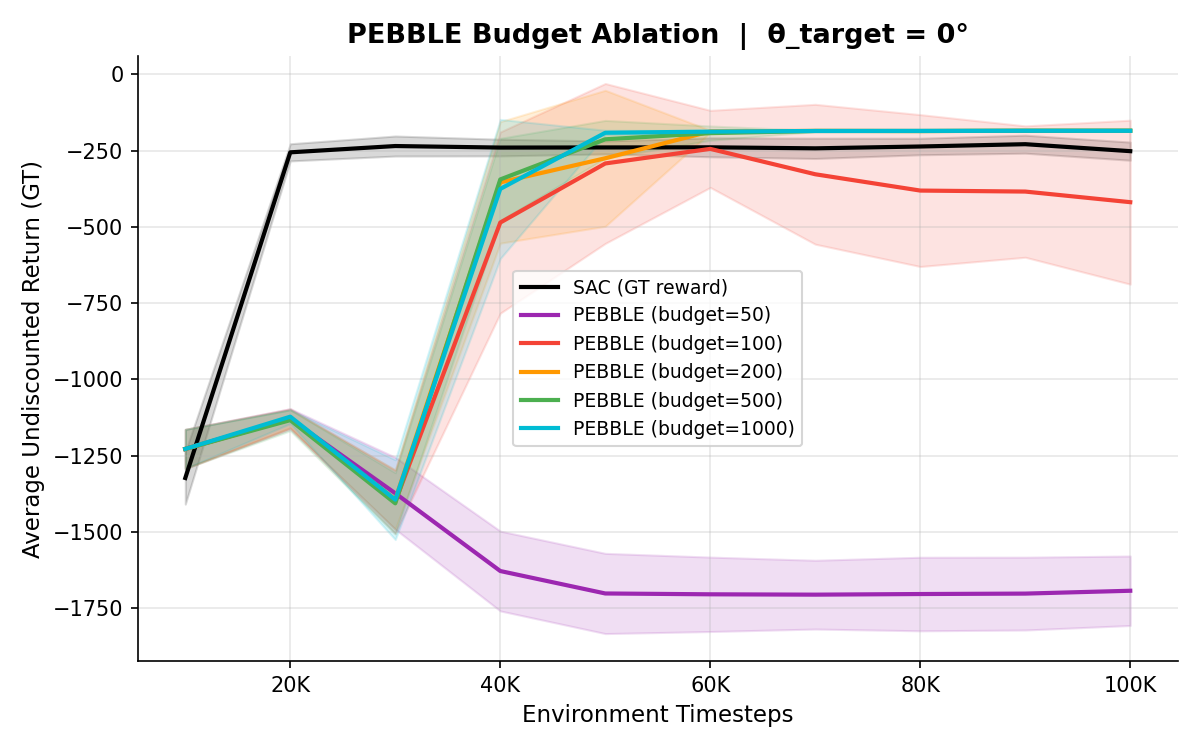
\includegraphics[width=\linewidth]{images/pebble_budget_ablation_theta0.png}
            \caption*{$\theta_{\text{target}}=0^\circ$}
        \end{minipage}\hfill
        \begin{minipage}{0.32\textwidth}
            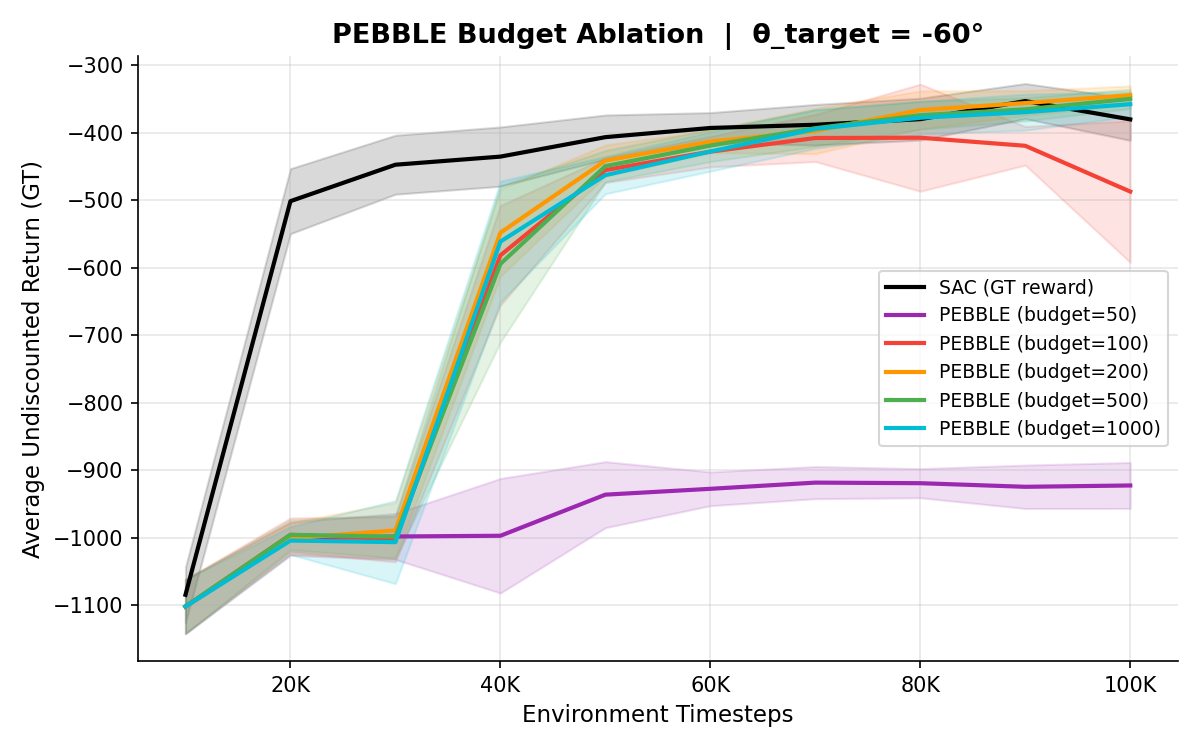
\includegraphics[width=\linewidth]{images/pebble_budget_ablation_theta-60.png}
            \caption*{$\theta_{\text{target}}=-60^\circ$}
        \end{minipage}\hfill
        \begin{minipage}{0.32\textwidth}
            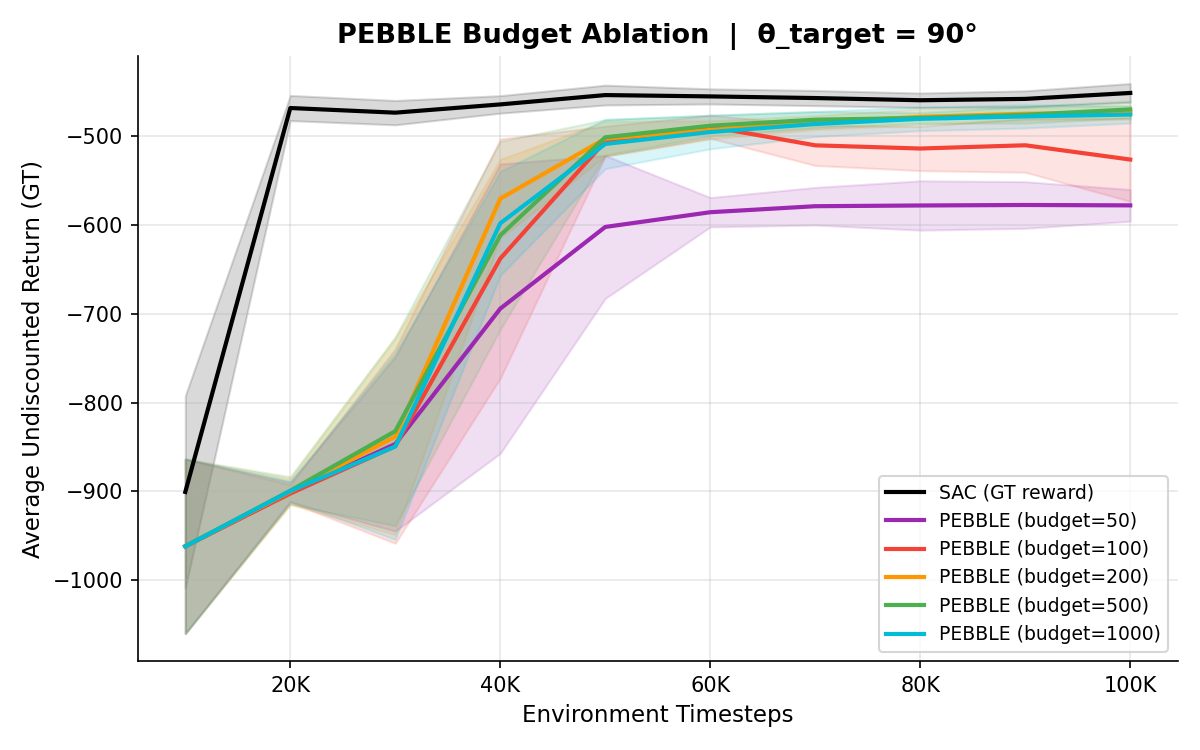
\includegraphics[width=\linewidth]{images/pebble_budget_ablation_theta90.png}
            \caption*{$\theta_{\text{target}}=90^\circ$}
        \end{minipage}\\[4pt]
        \begin{minipage}{0.32\textwidth}
            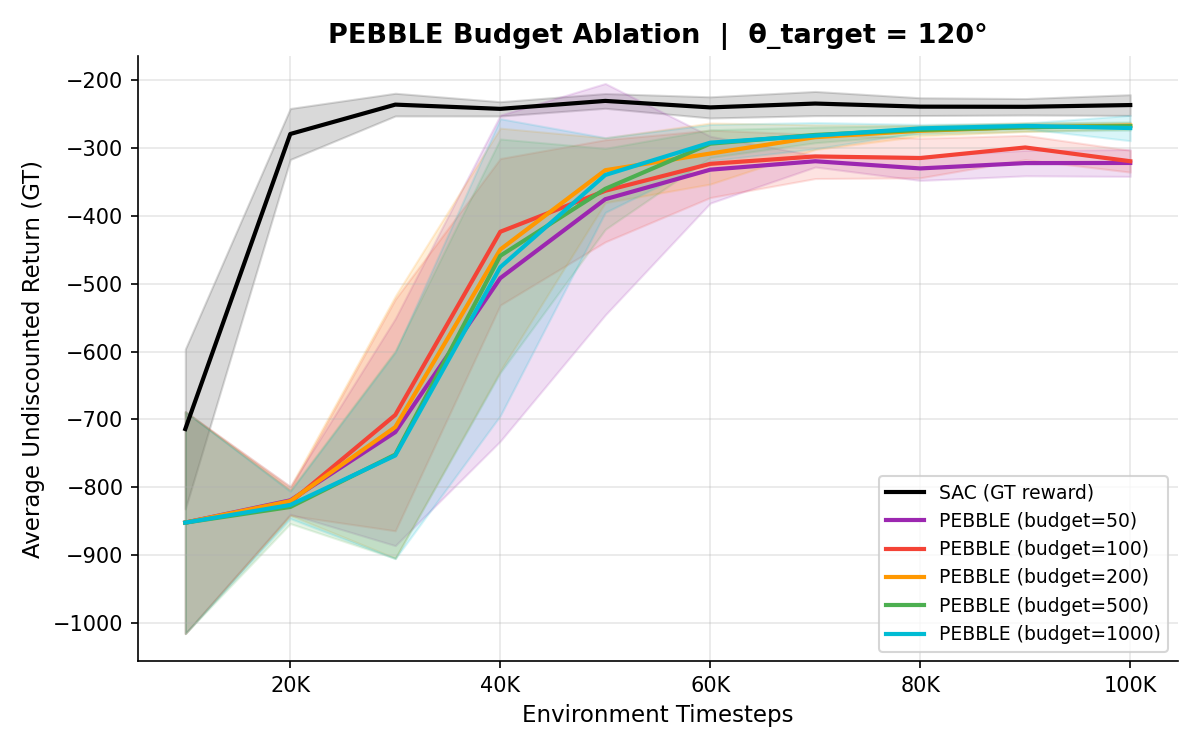
\includegraphics[width=\linewidth]{images/pebble_budget_ablation_theta120.png}
            \caption*{$\theta_{\text{target}}=120^\circ$}
        \end{minipage}\hfill
        \begin{minipage}{0.32\textwidth}
            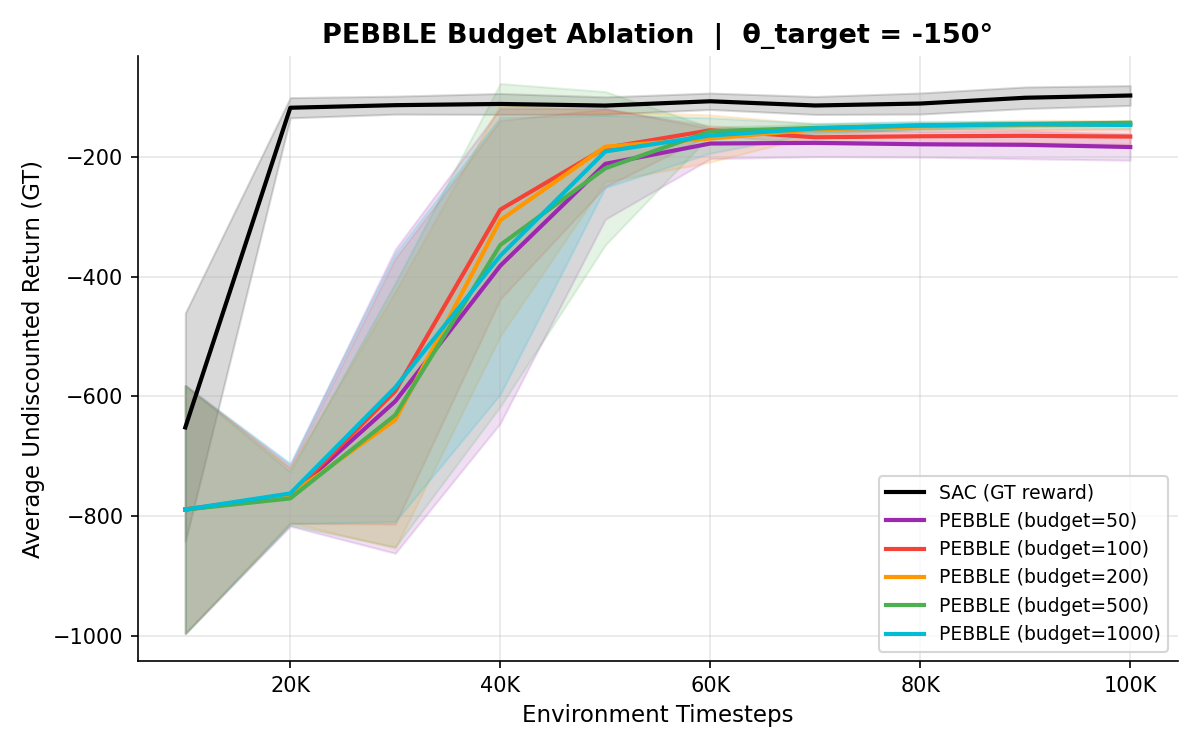
\includegraphics[width=\linewidth]{images/pebble_budget_ablation_theta-150.png}
            \caption*{$\theta_{\text{target}}=-150^\circ$}
        \end{minipage}\hfill
        \begin{minipage}{0.32\textwidth}\centering\vfill SAC-GT shown in black for reference; PEBBLE for $B\in\{50,100,200,500,1000\}$.\vfill\end{minipage}
        \caption{PEBBLE feedback-budget ablation on Pendulum-v1, mean $\pm$ std over $15$ seeds.}
        \label{fig:pebble_budget}
    \end{figure}

    \textbf{Observations.}
    \begin{itemize}
        \item \emph{$B=50$ is catastrophic on dense-reward targets.} On $\theta=0$ the $B=50$ runs actively \emph{diverge} (final return $\approx -1700$), worse than the random warm-up policy. With so few labels the learned reward never resolves which states are near the target, so the policy chases the noisy reward gradient into bad regions of state space. The effect is the same in spirit at $\theta=-60$ (stuck at $\approx -920$, $\sim 2.5\times$ worse than SAC-GT) and $\theta=90$ ($\approx -580$ vs $-453$ for SAC-GT). Targets with strong gravitational shaping ($\theta=120,-150$) are more robust because even a coarse learned reward agrees with gravity, but $B=50$ still trails the higher budgets at the end.
        \item \emph{$B=100$ is the smallest budget that learns reliably.} It recovers most of the SAC-GT performance ($\theta=0$: $-419$ vs $-185$ for $B\geq 200$ -- noisier and a clear final gap; $\theta=-60$: $-487$ vs $-352$; other targets: within $\sim 50$ of the best).
        \item \emph{$B\in\{200,500,1000\}$ are statistically indistinguishable across all five targets} (e.g.\ $\theta=0$: $-185\pm 1$ for all three; $\theta=-60$: $-344$ vs $-349$ vs $-357$; $\theta=90$: $-474$ vs $-470$ vs $-476$). This is consistent with the query schedule: once the budget exceeds the natural cap of $\sim 200$ queries imposed by the $2$K-step query interval over $100$K training steps, additional budget cannot be consumed and the curves collapse onto a single line.
        \item \emph{Sample-efficiency in preference space scales with reward difficulty.} Targets with high reward density and reliable gradient information ($\theta=-150$) tolerate small budgets ($B=50$ still reaches $-184$, only $\sim 75$ worse than SAC-GT). Targets where the reward landscape is sharply peaked and requires fine resolution ($\theta=0,-60$) need substantially more labels to escape early misspecification.
    \end{itemize}

    \textbf{Take-away.} For $100$K-step Pendulum training, $\approx 200$ preference labels are sufficient to match SAC-GT to within $5$--$15\%$ of the final return on every target, $100$ labels are a usable but noisier minimum, and $50$ labels are insufficient and can be actively harmful. Practically, the useful knob is not ``how much budget'' once it exceeds $\sim 200$, but ``how often does the trainer query''; spending labels earlier in training (where the learned reward bootstraps policy learning) yields most of the return gain.
\end{enumerate}

\end{document}


